%%%%%%%%%%%%%%%%%%%%%%%%%%%%%%%%%%%%%%%%%%%%%%%%%%
\section{Experiments}
\label{main:sec:experiments}
%%%%%%%%%%%%%%%%%%%%%%%%%%%%%%%%%%%%%%%%%%%%%%%%%%

We provide extensive experimental results to show how \gls{mpnp} and \gls{mpanp} effectively increase performance upon the following baselines: \gls{cnp}, \gls{np}, \gls{bnp}, \gls{canp}, \gls{anp}, and \gls{banp}. All models except deterministic models (i.e., \gls{cnp} and \gls{canp}) use the same number of samples; $K=5$ for the image completion task and $K=10$ for the others. Refer to~\cref{app:sec:architectures,app:sec:details} for more detailed experimental setup including model architectures, dataset and evaluation metrics.

% In this section, we carry out various experiments to show how \gls{mpnp} effectly increase performance.
% We compare our model (\gls{mpnp} and \gls{mpanp}) with various baseline \gls{npf} models(\gls{cnp}, \gls{np}, \gls{bnp}, \gls{neubnp}, \gls{canp}, \gls{anp}, \gls{banp} and \gls{neubanp}).
% We used same number of samples($K=5$ for image completion task and $K=10$ for the others) for all models except deterministic models \gls{cnp} and \gls{canp}.
% For detailed experimental setup including model architectures and dataset, please refer to \cref{app:sec:architectures,app:sec:details}.

%%%%%%%%%%%%%%%%%%%%%%%%%%%%%%%%%%%%%%%%%%%%%%%%%%
\subsection{1D Regression}
\label{main:sec:experiments:1dregression}

In this section, we conducted 1D regression experiments following \citet{kim2018attentive} and \citet{lee2020bootstrapping}. 
In this experiments, the dataset curves are generated from \gls{gp} with 4 different settings: \romannumeral1) RBF kernels, \romannumeral2) Mat\'ern 5/2 kernels, \romannumeral3) Periodic kernels, and \romannumeral4) RBF kernels with Student's $t$ noise.

\paragraph{Infinite Training Dataset}
\label{main:subsec:infinite_training}
\begin{figure}[t]
    \centering
    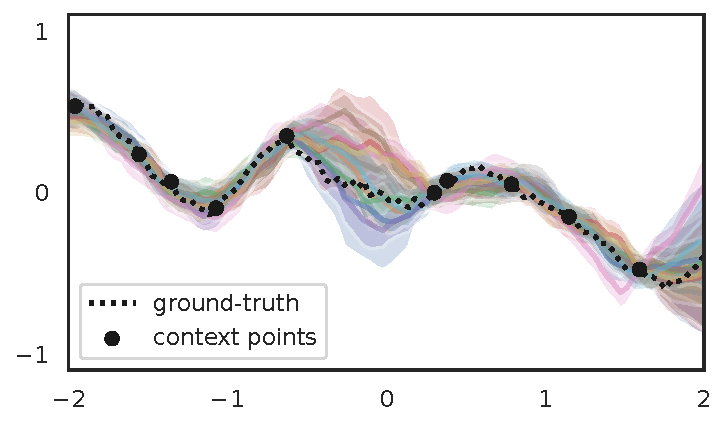
\includegraphics[width = 0.49\textwidth]{figure/main_vis_1.pdf}
    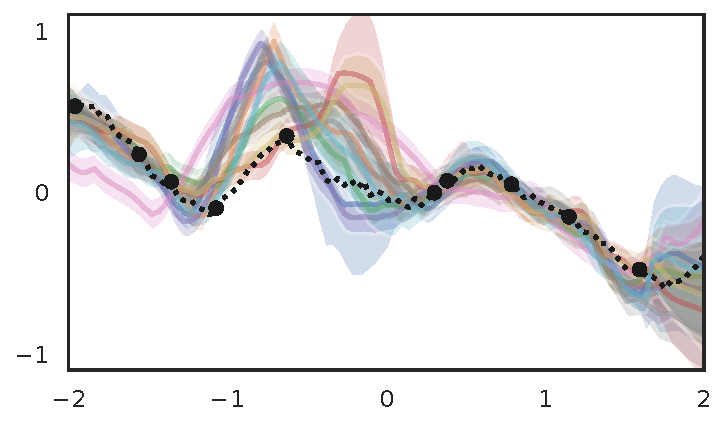
\includegraphics[width = 0.49\textwidth]{figure/main_vis_2.pdf}
    % \includegraphics[width = 0.32\textwidth]{figure/data plot 9.pdf}
    % \includegraphics[width = 0.32\textwidth]{figure/sample plot 9.pdf}
    % \includegraphics[width = 0.32\textwidth]{figure/posterior plot 9.pdf}
    \caption{Posterior samples of \gls{mpanp} for 1D regression task with RBF kernel. The black dashed line is the true function sampled from \gls{gp} with RBF kernel, and the black dots are context points. We visualized decoded mean and standard deviation with colored lines and areas. (Left) \Gls{mpanp} posterior predictions using the combined features of the original contexts and the generated pseudo contexts. (Right) Predictions using only the generated pseudo contexts without the original contexts. The pseudo contexts are decoded into reasonable functions, especially with high uncertainty for the region without context points.}
    % \caption{\color{blue}It shows posterior samples of \gls{mpanp} with context data and generated pseudo context data in 1D regression task with RBF kernel. Here, the black dashed line is a function sampled from \gls{gp} with RBF kernel and the black dots are context points. (Left) Overlaid posterior predictions with the combined feature from the contexts and generated pseudo contexts. Colored lines and areas represent decoded mean and std. (Right) In order to show the quality of generated pseudo context dataset, we visualize the posterior predictions with feature only from the generated pseudo contexts.}
    % \caption{Generated pseudo context data and posterior samples of MPANP in 1d regression task. (Left)
    % We train an autoencoder that can decode the representations $R_c$ into the points in the input space, and visualize the decoded inputs of the generated pseudo-contexts using the autoencoder. Red crosses are the real context data points, and the points sharing the same colors correspond to a set of pseudo context. (Right) Overlaid posterior predictions from the generated pseudo contexts.} 
    \label{fig:feature_method}
\end{figure}

% \begin{table}[t]
%     \caption{Context and target log likelihood values on data sampled from Gaussian Processes with various kernel. In the last column $t$-noise data generated by adding noise sampled from student $t$ distribution to Gaussian Processes with RBF Kernel. Performances are measured over 4 seeds.}
%     \label{tab:table_1d}
%     \centering
%     \scriptsize
%     \resizebox{\textwidth}{!}{
%     \begin{tabular}{lrrrrrrrrrr}
%     \toprule
%          Dataset             &               & RBF           &               &Matern         &               & Periodic       &               &t-noise \\
%         \midrule                  
%                              & context       & target        & context       & target        & context       & target         & context       & target  \\
%                 \midrule
%  CNP                 & $0.971\pm{0.004}$ & $0.266\pm{0.007}$ & $0.855\pm{0.001}$ & $0.105\pm{0.008}$ &$-0.151\pm{0.020}$ & $-0.722\pm{0.010}$ &$-0.005\pm{0.054}$ & $-0.583\pm{0.009}$ \\
%  BNP                 & $0.978\pm{0.018}$ & $0.307\pm{0.010}$ & $0.880\pm{0.006}$ & $0.153\pm{0.007}$ &$-0.086\pm{0.016}$ & $-0.703\pm{0.003}$ &$ 0.000\pm{0.059}$ & $-0.434\pm{0.012}$  \\
%  NeuBNP              & $0.903\pm{0.005}$ & $0.248\pm{0.006}$ & $0.779\pm{0.012}$ & $0.091\pm{0.005}$ &$-0.084\pm{0.010}$ & $-0.691\pm{0.013}$ &$ 0.024\pm{0.081}$ & $-0.487\pm{0.043}$  \\+

%  Ours                & $\textbf{1.102}\pm{0.008}$ & $\textbf{0.446}\pm{0.007}$ & $\textbf{1.021}\pm{0.004}$ & $\textbf{0.264}\pm{0.008}$ &$ \textbf{0.174}\pm{0.026}$ & $\textbf{-0.676}\pm{0.007}$ &$ \textbf{0.205}\pm{0.047}$ & $\textbf{-0.364}\pm{0.008}$  \\
%         \midrule
%  AttnCNP              & $1.372\pm{0.002}$ & $0.575\pm{0.021}$ & $1.371\pm{0.004}$ & $0.396\pm{0.004}$ & $\textbf{1.229}\pm{0.028}$ & $-0.711\pm{0.015}$ & $0.415\pm{0.031}$ & $-0.783\pm{0.046}$ \\
%  AttnBNP              & $1.372\pm{0.001}$ & $0.644\pm{0.008}$ & $1.372\pm{0.001}$ & $0.462\pm{0.010}$ & $0.776\pm{0.001}$ & $-0.876\pm{0.034}$ & $0.813\pm{0.023}$ & $-0.489\pm{0.027}$  \\
%  AttnNeuBNP           & $1.353\pm{0.003}$ & $0.601\pm{0.002}$ & $1.341\pm{0.003}$ & $0.417\pm{0.011}$ & $0.626\pm{0.004}$ & $-0.744\pm{0.007}$ & $0.748\pm{0.039}$ & $\textbf{-0.391}\pm{0.012}$  \\
%  Ours                 & $\textbf{1.375}\pm{0.000}$ & $\textbf{0.686}\pm{0.003}$ & $\textbf{1.374}\pm{0.000}$ & $\textbf{0.487}\pm{0.002}$ & $1.168\pm{0.036}$ & $\textbf{-0.662}\pm{0.029}$ & $\textbf{0.887}\pm{0.055}$ & $-0.476\pm{0.031}$  \\
%         \bottomrule
%     \end{tabular}}
% \end{table}

% \begin{table}[t]
    \caption{Context and target log likelihood values on data sampled from Gaussian Processes with various kernel. In the last column $t$-noise data generated by adding noise sampled from student $t$ distribution to Gaussian Processes with RBF Kernel. Performances are measured over 4 seeds.\\}
    \label{tab:table_gp_inf}
    \centering
    \scriptsize
    \renewcommand{\arraystretch}{0.9}
    \resizebox{0.95\textwidth}{!}{
    \begin{tabular}{lrrrrrrrrrrrr}
        \toprule
        \multirow{3}{*}{Model} & \multicolumn{2}{r}{RBF}                                   & \multicolumn{2}{r}{Matern}                                & \multicolumn{2}{r}{Periodic}                                & \multicolumn{2}{r}{$t$-noise}                               \\
                                 \cmidrule(lr){2-3}                                          \cmidrule(lr){4-5}                                          \cmidrule(lr){6-7}                                            \cmidrule(lr){8-9}
                               & context                     & target                      & context                     & target                      & context                      & target                       & context                      & target                       \\
        \midrule
CNP                    &         0.964  $\pm{0.006}$ &         0.288  $\pm{0.006}$ &         0.859  $\pm{0.009}$ &         0.124  $\pm{0.011}$ &         -0.139  $\pm{0.007}$ &         -0.742  $\pm{0.011}$ &         -0.012  $\pm{0.021}$ &         -0.760  $\pm{0.025}$ \\
NP                     &         0.953  $\pm{0.003}$ &         0.306  $\pm{0.004}$ &         0.842  $\pm{0.015}$ &         0.133  $\pm{0.008}$ &         -0.346  $\pm{0.026}$ &         -0.698  $\pm{0.007}$ &         -0.018  $\pm{0.022}$ &         -0.656  $\pm{0.028}$ \\
BNP                    &         1.020  $\pm{0.006}$ &         0.372  $\pm{0.006}$ &         0.929  $\pm{0.008}$ &         0.206  $\pm{0.006}$ &         -0.036  $\pm{0.031}$ &         -0.738  $\pm{0.011}$ &         -0.051  $\pm{0.051}$ &         -0.670  $\pm{0.023}$ \\
NeuBNP                 &         0.929  $\pm{0.011}$ &         0.275  $\pm{0.007}$ &         0.834  $\pm{0.008}$ &         0.122  $\pm{0.004}$ &         -0.231  $\pm{0.010}$ &         -0.785  $\pm{0.023}$ &          0.038  $\pm{0.009}$ &         -0.516  $\pm{0.018}$ \\
DirectNP               &         0.876  $\pm{0.005}$ &         0.260  $\pm{0.011}$ &         0.757  $\pm{0.013}$ &         0.099  $\pm{0.015}$ &         -0.242  $\pm{0.022}$ &         -0.696  $\pm{0.004}$ &         -0.202  $\pm{0.039}$ &         -0.651  $\pm{0.013}$ \\
MPNP (ours)            & \textBF{1.086} $\pm{0.005}$ & \textBF{0.457} $\pm{0.002}$ & \textBF{1.005} $\pm{0.014}$ & \textBF{0.278} $\pm{0.006}$ & \textBF{-0.017} $\pm{0.013}$ & \textBF{-0.681} $\pm{0.009}$ & \textBF{ 0.119} $\pm{0.025}$ & \textBF{-0.381} $\pm{0.013}$ \\
\cmidrule(lr){1-1}       \cmidrule(lr){2-3}                                          \cmidrule(lr){4-5}                                          \cmidrule(lr){6-7}                                            \cmidrule(lr){8-9}
CANP                   &         1.372  $\pm{0.000}$ &         0.611  $\pm{0.008}$ &         1.370  $\pm{0.001}$ &         0.423  $\pm{0.004}$ &          1.168  $\pm{0.051}$ &         -0.747  $\pm{0.037}$ &          0.404  $\pm{0.057}$ &         -1.036  $\pm{0.103}$ \\
ANP                    &         1.372  $\pm{0.003}$ &         0.617  $\pm{0.027}$ &         1.372  $\pm{0.001}$ &         0.432  $\pm{0.025}$ & \textBF{ 1.178} $\pm{0.054}$ &         -0.719  $\pm{0.024}$ &          0.708  $\pm{0.054}$ &         -0.728  $\pm{0.093}$ \\
BANP                   & \textBF{1.374} $\pm{0.001}$ &         0.663  $\pm{0.002}$ &         1.371  $\pm{0.002}$ &         0.472  $\pm{0.003}$ &          0.754  $\pm{0.083}$ &         -0.913  $\pm{0.028}$ &          0.477  $\pm{0.008}$ &         -0.660  $\pm{0.059}$ \\
NeuBANP                &         1.357  $\pm{0.002}$ &         0.651  $\pm{0.005}$ &         1.352  $\pm{0.002}$ &         0.473  $\pm{0.007}$ &          0.697  $\pm{0.022}$ &         -0.779  $\pm{0.013}$ &          0.670  $\pm{0.028}$ &         -0.450  $\pm{0.014}$ \\
DirectANP              &         1.353  $\pm{0.003}$ &         0.653  $\pm{0.010}$ &         1.342  $\pm{0.009}$ &         0.430  $\pm{0.030}$ &          1.109  $\pm{0.118}$ &         -0.632  $\pm{0.031}$ &          0.254  $\pm{0.023}$ &         -0.781  $\pm{0.033}$ \\
MPANP (ours)           & \textBF{1.374} $\pm{0.000}$ & \textBF{0.698} $\pm{0.007}$ & \textBF{1.373} $\pm{0.001}$ & \textBF{0.501} $\pm{0.005}$ &          1.167  $\pm{0.047}$ & \textBF{-0.628} $\pm{0.027}$ & \textBF{ 0.773} $\pm{0.039}$ & \textBF{-0.446} $\pm{0.057}$ \\
% CNP                    &         0.964  $\pm{0.006}$ &         0.288  $\pm{0.006}$ &         0.859  $\pm{0.009}$ &         0.124  $\pm{0.011}$ &         -0.139  $\pm{0.007}$ &         -0.742  $\pm{0.011}$ &         -0.012  $\pm{0.021}$ &         -0.760  $\pm{0.025}$ \\
% NP                     &         0.953  $\pm{0.003}$ &         0.306  $\pm{0.004}$ &         0.842  $\pm{0.015}$ &         0.133  $\pm{0.008}$ &         -0.346  $\pm{0.026}$ &         -0.698  $\pm{0.007}$ &         -0.018  $\pm{0.022}$ &         -0.656  $\pm{0.028}$ \\
% BNP                    &         1.020  $\pm{0.006}$ &         0.372  $\pm{0.006}$ &         0.929  $\pm{0.008}$ &         0.206  $\pm{0.006}$ &         -0.036  $\pm{0.031}$ &         -0.738  $\pm{0.011}$ &         -0.051  $\pm{0.051}$ &         -0.670  $\pm{0.023}$ \\
% NeuBNP                 &         0.929  $\pm{0.011}$ &         0.275  $\pm{0.007}$ &         0.834  $\pm{0.008}$ &         0.122  $\pm{0.004}$ &         -0.231  $\pm{0.010}$ &         -0.785  $\pm{0.023}$ &          0.038  $\pm{0.009}$ &         -0.516  $\pm{0.018}$ \\
% MPNP (ours)            & \textBF{1.086} $\pm{0.005}$ & \textBF{0.457} $\pm{0.002}$ & \textBF{1.005} $\pm{0.014}$ & \textBF{0.278} $\pm{0.006}$ & \textBF{-0.017} $\pm{0.013}$ & \textBF{-0.681} $\pm{0.009}$ & \textBF{ 0.119} $\pm{0.025}$ & \textBF{-0.381} $\pm{0.013}$ \\
% \cmidrule(lr){1-1}       \cmidrule(lr){2-3}                                          \cmidrule(lr){4-5}                                          \cmidrule(lr){6-7}                                            \cmidrule(lr){8-9}
% CANP                   &         1.372  $\pm{0.000}$ &         0.611  $\pm{0.008}$ &         1.370  $\pm{0.001}$ &         0.423  $\pm{0.004}$ &          1.168  $\pm{0.051}$ &         -0.747  $\pm{0.037}$ &          0.404  $\pm{0.057}$ &         -1.036  $\pm{0.103}$ \\
% ANP                    &         1.372  $\pm{0.003}$ &         0.617  $\pm{0.027}$ &         1.372  $\pm{0.001}$ &         0.432  $\pm{0.025}$ & \textBF{1.178}  $\pm{0.054}$ &         -0.719  $\pm{0.024}$ &          0.708  $\pm{0.054}$ &         -0.728  $\pm{0.093}$ \\
% BANP                   & \textBF{1.374} $\pm{0.001}$ &         0.663  $\pm{0.002}$ &         1.371  $\pm{0.002}$ &         0.472  $\pm{0.003}$ &          0.754  $\pm{0.083}$ &         -0.913  $\pm{0.028}$ &          0.477  $\pm{0.008}$ &         -0.660  $\pm{0.059}$ \\
% NeuBANP                &         1.357  $\pm{0.002}$ &         0.651  $\pm{0.005}$ &         1.352  $\pm{0.002}$ &         0.473  $\pm{0.007}$ &          0.697  $\pm{0.022}$ &         -0.779  $\pm{0.013}$ &          0.670  $\pm{0.028}$ &         -0.450  $\pm{0.014}$ \\
% MPANP (ours)           & \textBF{1.374} $\pm{0.000}$ & \textBF{0.698} $\pm{0.007}$ & \textBF{1.373} $\pm{0.001}$ & \textBF{0.501} $\pm{0.005}$ &         1.167 $\pm{0.047}$ & \textBF{-0.628} $\pm{0.027}$ & \textBF{ 0.773} $\pm{0.039}$ & \textBF{-0.446} $\pm{0.057}$ \\
        \bottomrule
    \end{tabular}}
\end{table}
\begin{table}[t]
\centering
\caption{Test results for 1D regression tasks on RBF, Matern, Periodic, and $t$-noise. `Context' and `Target' respectively denote context and target log-likelihood values. All values are averaged over four seeds. See~\cref{table/app_gp_inf_full} for the task log-likelihood values.}
\label{table/main_gp_inf}
\resizebox{\linewidth}{!}{
\begin{tabular}{lrrrrrrrr}
\toprule
      & \multicolumn{2}{c}{RBF} & \multicolumn{2}{c}{Matern} & \multicolumn{2}{c}{Periodic} & \multicolumn{2}{c}{$t$-noise} \\
\cmidrule(lr){2-3}\cmidrule(lr){4-5}\cmidrule(lr){6-7}\cmidrule(lr){8-9}
Model & Context & Target & Context & Target & Context & Target & Context & Target \\
\midrule
CNP & 
 1.096$\spm{0.023}$ &  0.515$\spm{0.018}$ &
 1.031$\spm{0.010}$ &  0.347$\spm{0.006}$ &
-0.120$\spm{0.020}$ & -0.729$\spm{0.004}$ &
 0.032$\spm{0.014}$ & -0.816$\spm{0.032}$ \\
NP & 
 1.022$\spm{0.005}$ &  0.498$\spm{0.003}$ &
 0.948$\spm{0.006}$ &  0.337$\spm{0.005}$ &
-0.267$\spm{0.024}$ & \textBF{-0.668}$\spm{0.006}$ &
 \textBF{0.201}$\spm{0.025}$ & -0.333$\spm{0.078}$ \\
BNP & 
 1.112$\spm{0.003}$ &  0.588$\spm{0.004}$ &
 1.057$\spm{0.009}$ &  0.418$\spm{0.006}$ &
-0.106$\spm{0.017}$ & -0.705$\spm{0.001}$ &
-0.009$\spm{0.032}$ & -0.619$\spm{0.191}$ \\
\textBF{MPNP (ours)} & 
 \textBF{1.189}$\spm{0.005}$ &  \textBF{0.675}$\spm{0.003}$ &
 \textBF{1.123}$\spm{0.005}$ &  \textBF{0.481}$\spm{0.007}$ &
 \textBF{0.205}$\spm{0.020}$ & \textBF{-0.668}$\spm{0.008}$ &
 0.145$\spm{0.017}$ & \textBF{-0.329}$\spm{0.025}$ \\
\midrule
CANP & 
 1.304$\spm{0.027}$ &  0.847$\spm{0.005}$ &
 1.264$\spm{0.041}$ &  0.662$\spm{0.013}$ &
 0.527$\spm{0.106}$ & -0.592$\spm{0.002}$ &
 0.410$\spm{0.155}$ & -0.577$\spm{0.022}$ \\
ANP & 
 \textBF{1.380}$\spm{0.000}$ &  0.850$\spm{0.007}$ &
 \textBF{1.380}$\spm{0.000}$ &  0.663$\spm{0.004}$ &
 0.583$\spm{0.011}$ & -1.019$\spm{0.023}$ &
 0.836$\spm{0.071}$ & -0.415$\spm{0.131}$ \\
BANP & 
 \textBF{1.380}$\spm{0.000}$ &  0.846$\spm{0.001}$ &
 \textBF{1.380}$\spm{0.000}$ &  0.662$\spm{0.005}$ &
 \textBF{1.354}$\spm{0.006}$ & -0.496$\spm{0.005}$ &
 0.646$\spm{0.042}$ & -0.425$\spm{0.050}$ \\
\textBF{MPANP (ours)} & 
 1.379$\spm{0.000}$ &  \textBF{0.881}$\spm{0.003}$ &
 \textBF{1.380}$\spm{0.000}$ &  \textBF{0.692}$\spm{0.003}$ &
 1.348$\spm{0.005}$ & \textBF{-0.494}$\spm{0.007}$ &
 \textBF{0.842}$\spm{0.062}$ & \textBF{-0.332}$\spm{0.026}$ \\
\bottomrule
\end{tabular}}
\end{table}


% \begin{figure}[t]
%     \centering
%     % 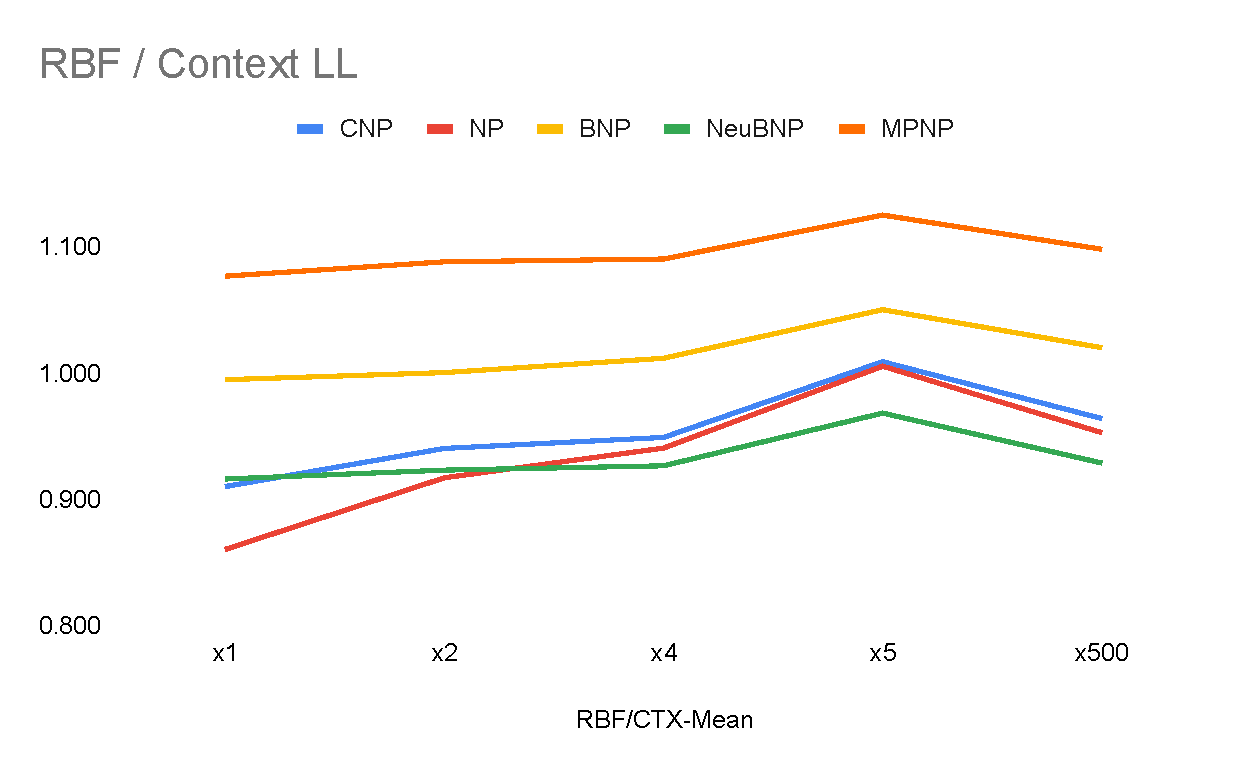
\includegraphics[width=0.24\textwidth]{figure/gp_finite/rbf_ctx_cnps.pdf}
%     % 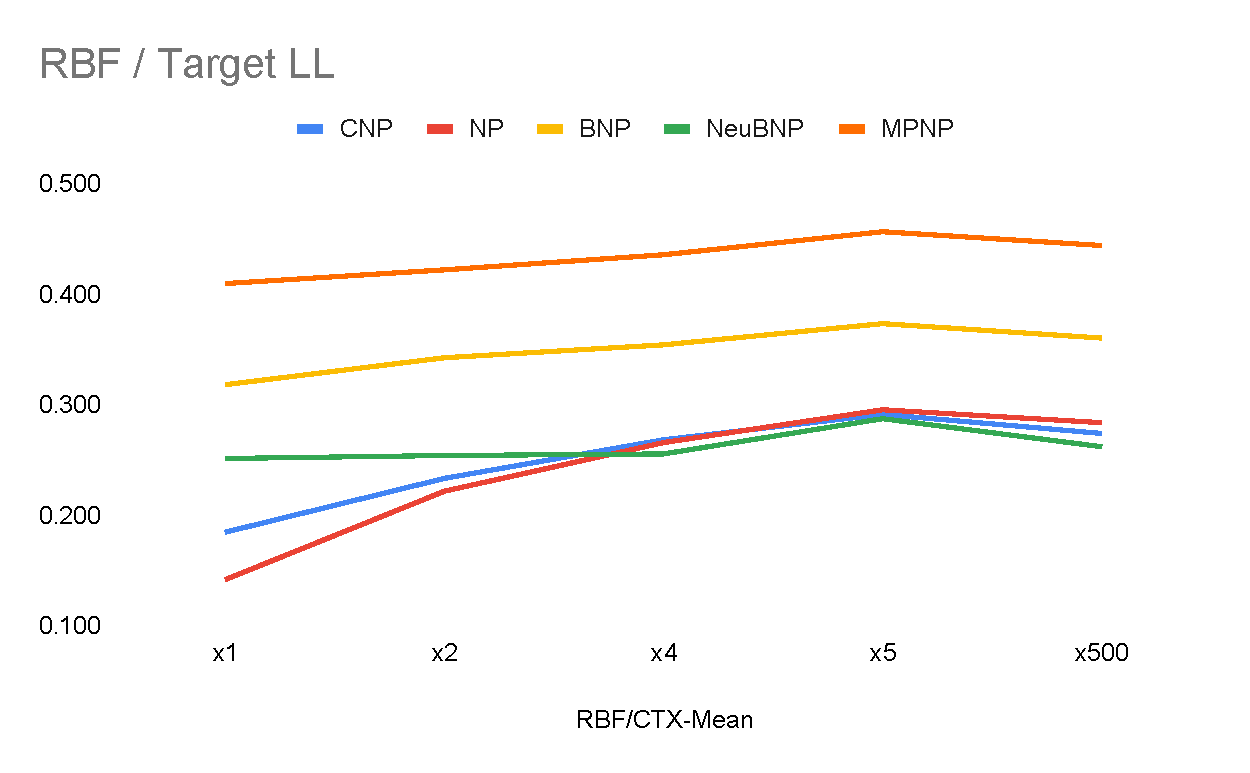
\includegraphics[width=0.24\textwidth]{figure/gp_finite/rbf_tar_cnps.pdf}
%     % 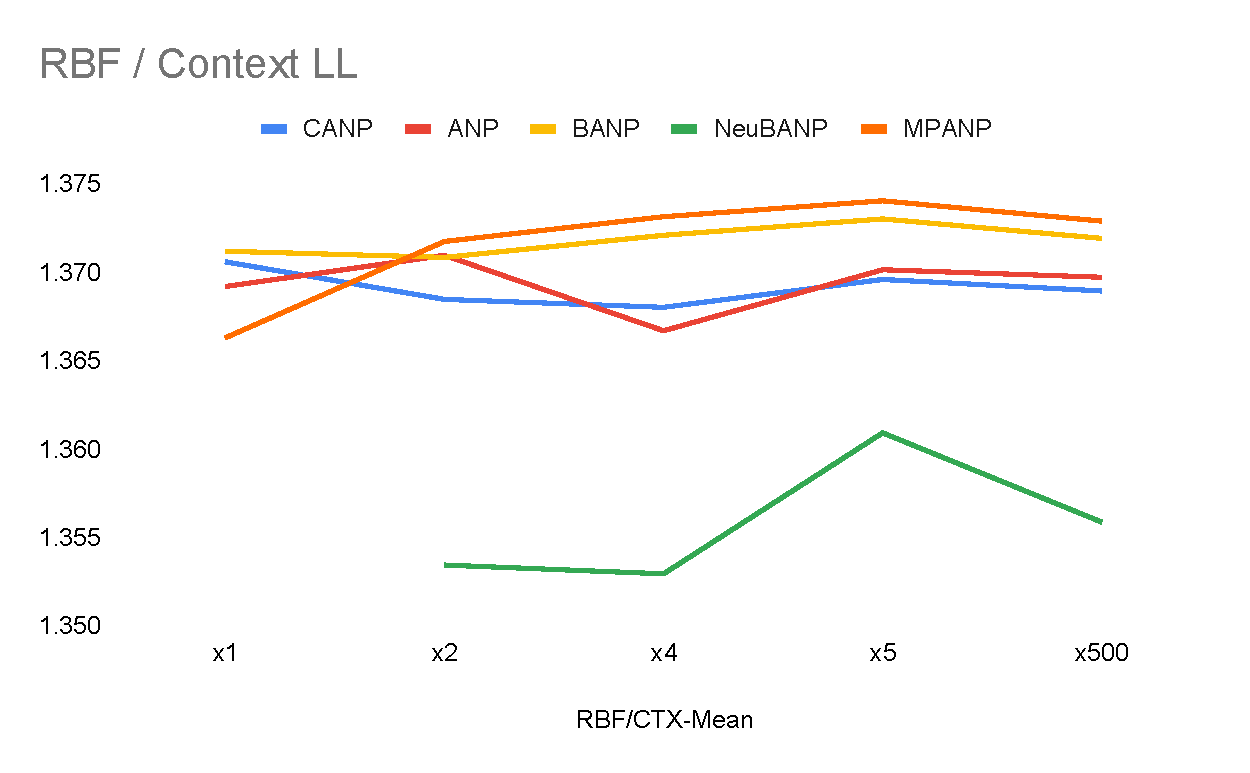
\includegraphics[width=0.24\textwidth]{figure/gp_finite/rbf_ctx_canps.pdf}
%     % 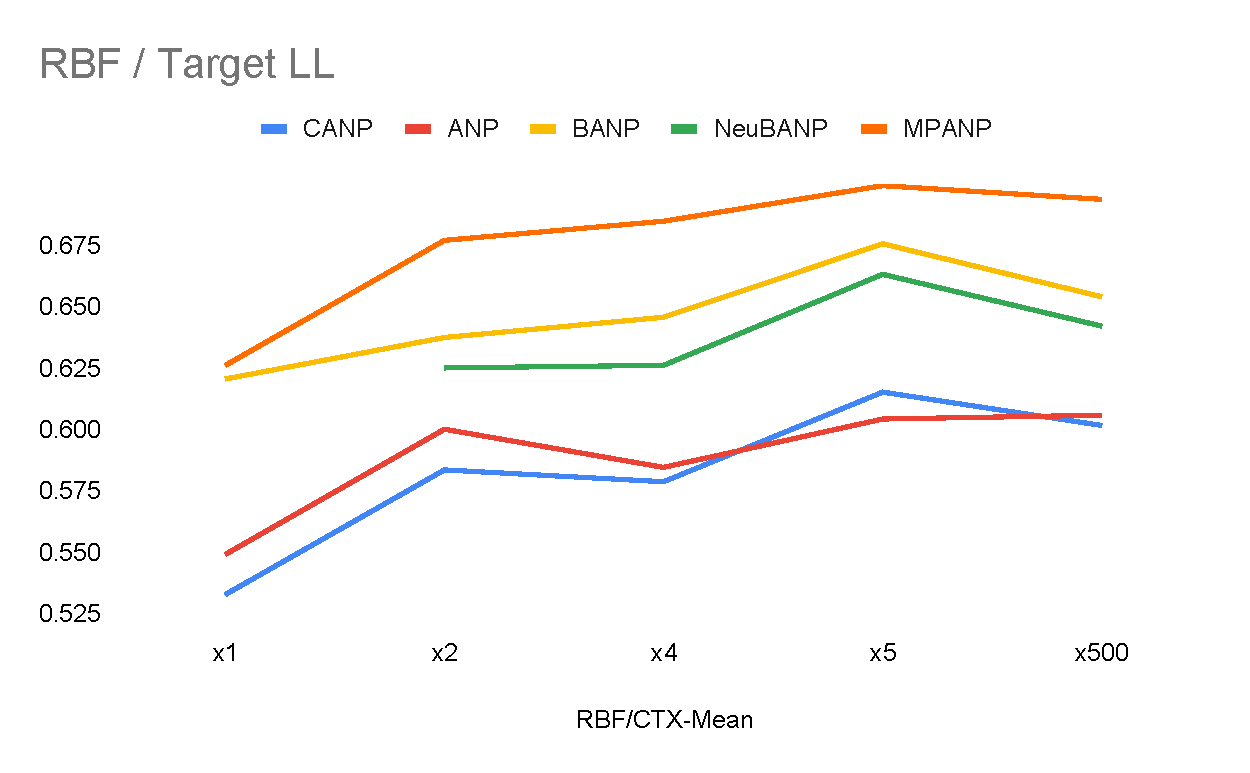
\includegraphics[width=0.24\textwidth]{figure/gp_finite/rbf_tar_canps.pdf}
%     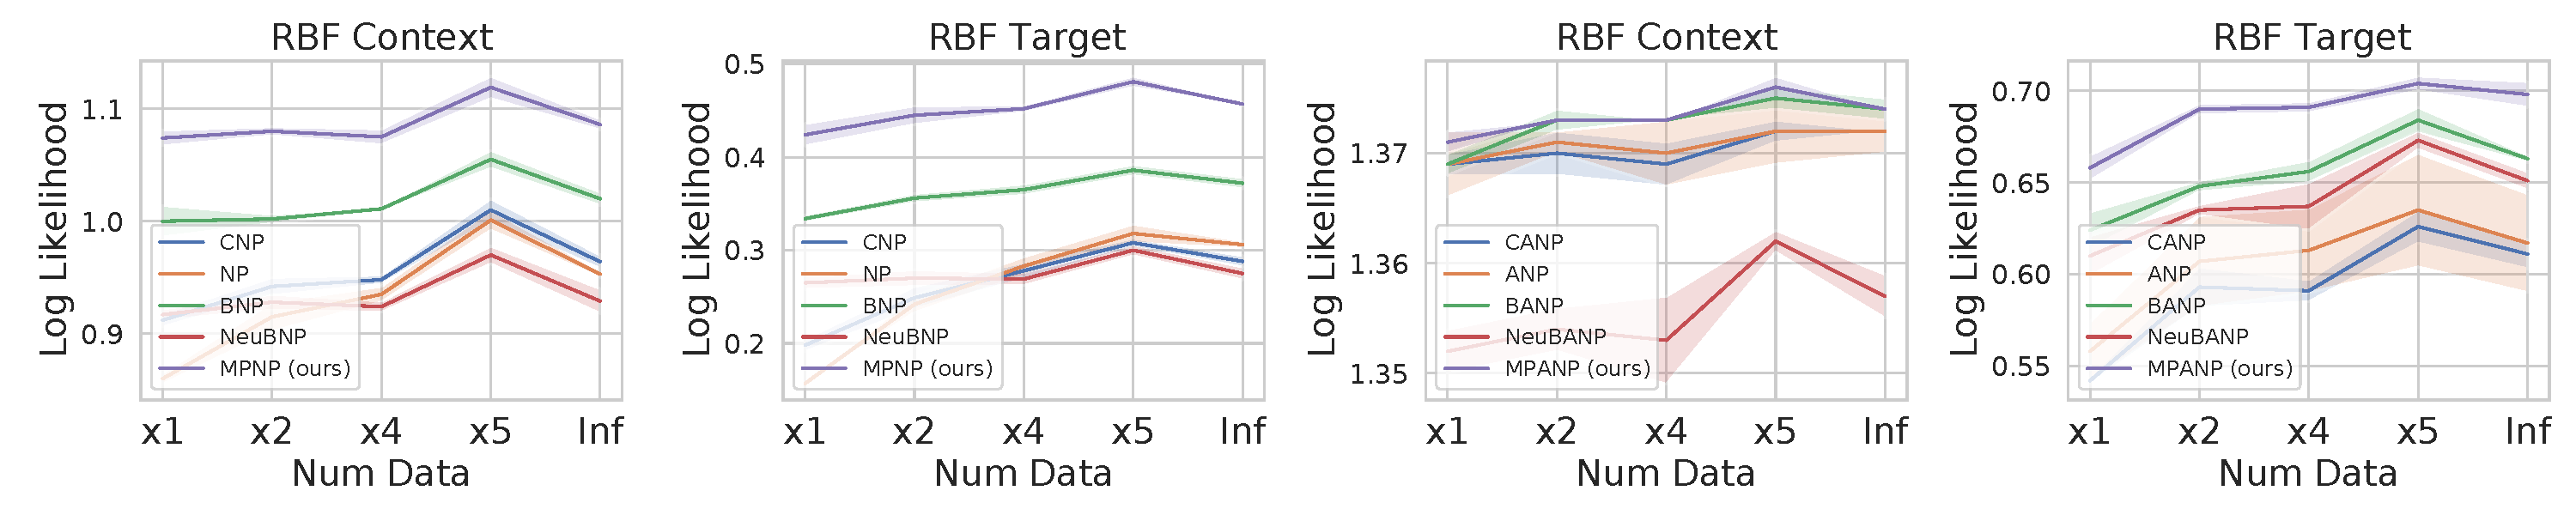
\includegraphics[width=\textwidth]{figure/finite.pdf}
%     \caption{Context and target log likelihood values of 1D regression experiments with RBF kernel. 
%     $\times n$ in the $x$ axis denotes how many times training data is used based on the number of training data of 500 epochs.
%     The first and the second figure are context and target log likelihood for \gls{cnp} variation models, respectively. The third and the forth are context and target log likelihood for \gls{canp} variation models, respectively.
% }
%     \label{fig:figure_gp_finite}
% \end{figure}
\begin{figure}[t]
    \centering
    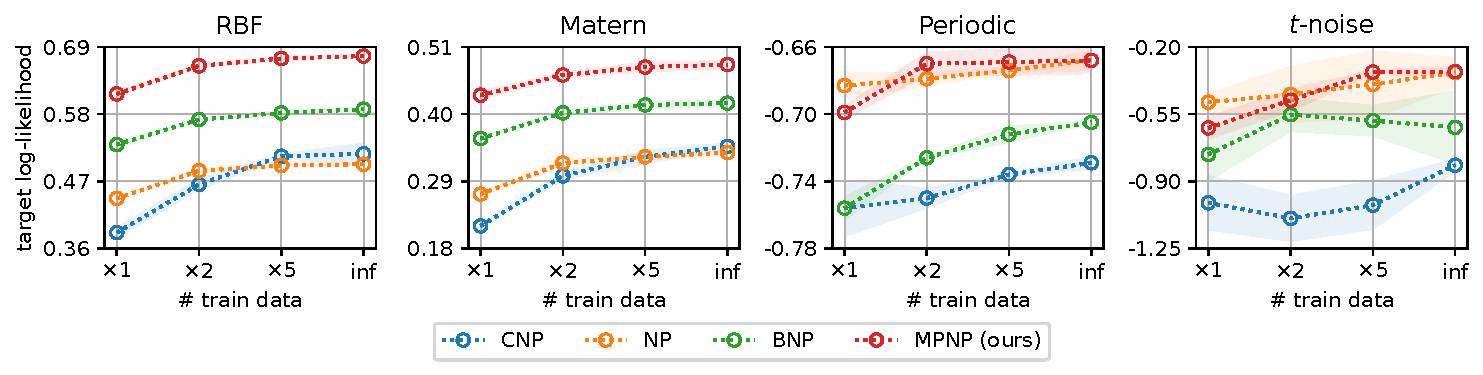
\includegraphics[width=0.95\textwidth]{figure/main_gp_finite_np.pdf}
    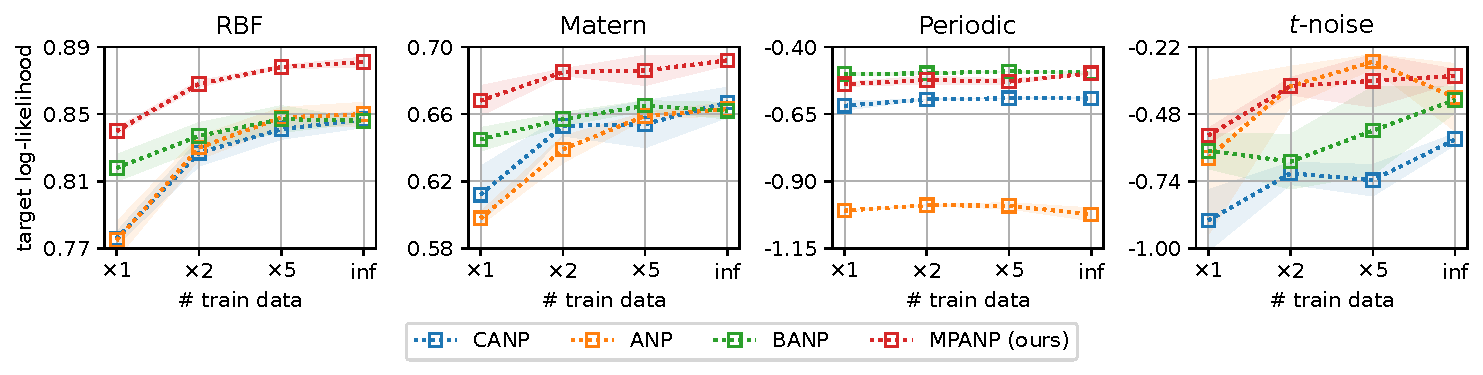
\includegraphics[width=0.95\textwidth]{figure/main_gp_finite_anp.pdf}
    \caption{Test target log-likelihood values with varying the number of train data for 1D regression tasks on RBF, Matern, Periodic, and $t$-noise. Here, x-axis denotes how many examples are used for training, i.e., $\times1$, $\times2$, and $\times5$ respectively denote $51200$, $102400$, and $256000$ train examples.}
    \label{figure/main_gp_finite}
\end{figure}

Previous works~\citep{garnelo2018neural,kim2018attentive,le2018empirical} assumed that there exists a \gls{gp} curve generator that can provide virtually infinite amount of tasks for training. We first follow this setup, training all models for 100,000 steps where a new task is generated from each training step. We compare the models by picking checkpoints achieving the lowest validation loss. \cref{table/main_gp_inf} clearly shows that our model outperforms the other models in most cases. This results show that our model well captures the functional uncertainty compared to the other methods.
In~\cref{app:sec:additional_experiments}, we also report the comparison with the baselines with increased number of parameters to match the additional number of parameters introduced for the generator in our model, where ours still significantly outperforms the baselines.

% We also report the performances of our model generating pseudo contexts directly in the input space, denoted as DirectNP and DirectANP in \cref{table/main_gp_inf}. Unfortunately, DirectNP and DirectANP perform worse then ours when generating representations, presumably due to the difficulty of generating inputs that should be processed with nonlinear encoders and decoders. See \cref{app:sec:directly_generating_input} for the model architectures and the samples generated from DirectNP and DirectANP. In \cref{fig:feature_method}, we present the generated pseudo context data and posterior samples from trained \gls{mpanp} model. 
% In \cref{app:sec:additional_experiments}, we also report the comparison with the baselines with increased number of parameters to match the additional number of parameters introduced for the generator in our model, where ours still significantly outperforms the baselines.

\paragraph{Finite Training Dataset}
We also compare the models on more realistic setting assuming a finite amount of training tasks. Specifically, we first configured the finite training dataset consisting of $\{51200, 102400, 256000\}$ examples at the start of the training, instead of generating new tasks for each training step. We then trained all models with the same 100,000 training iterations in order to train the models with the same training budget as in the infinite training dataset situation. \cref{figure/main_gp_finite} clearly shows that our model consistently outperforms other models in terms of the target log-likelihood even when the training dataset is finite. This indicates that \glspl{mpnp} effectively learn a predictive distribution of unseen dataset from a given dataset with small number of tasks. Refer to~\cref{app:sec:additional_experiments} for more detailed results.

% Now we compare the models on more realistic setting assuming a finite amount of training tasks.
% In order to train the models with the same training budget as in the infinite training dataset situation, we first configured the training dataset so that 500 epochs become 100000 steps.
% We then gradually increase the number of data so that 100000 steps become 250, 125, and 100 epochs, respectively.
% \cref{fig:figure_gp_finite} shows that our model consistently outperforms other models for almost all dataset size in \gls{gp} with RBF kernel. This shows that \glspl{mpnp} effectively learn a predictive distribution of unseen dataset from a given dataset with small number of tasks. Please refer to \cref{app:sec:additional_experiments} for the results for the kernels other than RBF for which the results are similar as in RBF kernel.

% \paragraph{Robustness Across Kernels}
% \begin{table}[t]
    \caption{Results of Robustness among kernels experiments. Context and target log likelihood values on data sampled from Gaussian Processes with various kernels. Here we first trained models on RBF dataset and evaluate performances on various settings.  Performances are measured over 4 seeds.\\}
    \label{tab:table_gp_robust}
    \centering
    \scriptsize
    \renewcommand{\arraystretch}{0.85}
    \resizebox{\textwidth}{!}{
    \begin{tabular}{lrrrrrrrrrrrr}
        \toprule
        \multirow{3}{*}{Model} & \multicolumn{2}{r}{RBF}                                   & \multicolumn{2}{r}{Matern}                                & \multicolumn{2}{r}{Periodic}                                & \multicolumn{2}{r}{$t$-noise}                               \\
                                 \cmidrule(lr){2-3}                                          \cmidrule(lr){4-5}                                          \cmidrule(lr){6-7}                                            \cmidrule(lr){8-9}
                               & context                     & target                      & context                     & target                      & context                      & target                       & context                      & target                       \\
        \midrule
CNP                    &         0.964  $\pm{0.006}$ &         0.288  $\pm{0.006}$ &         0.826  $\pm{0.007}$ &         0.076  $\pm{0.007}$ &         -0.504  $\pm{0.045}$ &         -2.686  $\pm{0.087}$ &          0.151  $\pm{0.101}$ &         -2.382  $\pm{0.011}$ \\
NP                     &         0.951  $\pm{0.007}$ &         0.299  $\pm{0.007}$ &         0.804  $\pm{0.008}$ &         0.076  $\pm{0.015}$ &         -0.421  $\pm{0.011}$ &         -2.430  $\pm{0.110}$ &         -0.336  $\pm{1.016}$ &         -2.177  $\pm{0.157}$ \\
BNP                    &         1.020  $\pm{0.006}$ &         0.372  $\pm{0.006}$ &         0.890  $\pm{0.006}$ &         0.192  $\pm{0.007}$ & \textBF{-0.281} $\pm{0.004}$ & \textBF{-1.265} $\pm{0.009}$ &  \textBF{0.455} $\pm{0.001}$ & \textBF{-1.329} $\pm{0.092}$ \\
NeuBNP                 &         0.929  $\pm{0.011}$ &         0.275  $\pm{0.007}$ &         0.806  $\pm{0.012}$ &         0.109  $\pm{0.006}$ &         -0.378  $\pm{0.028}$ &         -1.730  $\pm{0.037}$ &          0.314  $\pm{0.077}$ &         -1.406  $\pm{0.184}$ \\
MPNP (ours)            & \textBF{1.086} $\pm{0.005}$ & \textBF{0.457} $\pm{0.002}$ & \textBF{0.967} $\pm{0.007}$ & \textBF{0.261} $\pm{0.005}$ &         -0.314  $\pm{0.026}$ &         -1.448  $\pm{0.025}$ &          0.104  $\pm{0.240}$ &         -1.638  $\pm{0.241}$ \\
\cmidrule(lr){1-1}       \cmidrule(lr){2-3}                                          \cmidrule(lr){4-5}                                          \cmidrule(lr){6-7}                                            \cmidrule(lr){8-9}
CANP                   &         1.372  $\pm{0.000}$ &         0.611  $\pm{0.008}$ &         1.367  $\pm{0.001}$ &         0.427  $\pm{0.006}$ &          0.312  $\pm{0.111}$ &         -6.607  $\pm{0.268}$ &          0.980  $\pm{0.045}$ &         -2.889  $\pm{0.094}$ \\
ANP                    &         1.372  $\pm{0.003}$ &         0.616  $\pm{0.026}$ &         1.367  $\pm{0.004}$ &         0.427  $\pm{0.028}$ &          0.445  $\pm{0.137}$ &         -6.521  $\pm{0.437}$ &          1.009  $\pm{0.025}$ &         -2.868  $\pm{0.120}$ \\
BANP                   & \textBF{1.374} $\pm{0.001}$ &         0.663  $\pm{0.002}$ &         1.370  $\pm{0.001}$ &         0.476  $\pm{0.006}$ &          0.731  $\pm{0.046}$ &         -3.165  $\pm{0.322}$ &          1.092  $\pm{0.011}$ &         -2.269  $\pm{0.170}$ \\
NeuBANP                &         1.357  $\pm{0.002}$ &         0.651  $\pm{0.005}$ &         1.347  $\pm{0.002}$ &         0.467  $\pm{0.007}$ & \textBF{ 0.970} $\pm{0.020}$ & \textBF{-2.300} $\pm{0.228}$ &  \textBF{1.169} $\pm{0.008}$ &         -2.090  $\pm{0.120}$ \\
MPANP (ours)           & \textBF{1.374} $\pm{0.000}$ & \textBF{0.699} $\pm{0.007}$ & \textBF{1.370} $\pm{0.001}$ & \textBF{0.500} $\pm{0.004}$ &          0.616  $\pm{0.042}$ &         -3.551  $\pm{0.092}$ &          1.016  $\pm{0.080}$ & \textBF{-2.071} $\pm{0.097}$ \\
        \bottomrule
    \end{tabular}}
\end{table}
% \citet{lee2020bootstrapping} conducted model-data mismatch experiments in 1D regression experiments by training the models with RBF kernels and evaluating them on the tasks generated from \glspl{gp} with kernels other than RBF.
% Following \citet{lee2020bootstrapping}, we first train a model with infinite \gls{gp} data with RBF kernel,
%  and measure the log-likelihoods on the test datasets generated from other kernels.
% As one can see from \cref{tab:table_gp_robust}, \glspl{mpnp} outperform baselines on RBF and Matern kernel (which is relatively simlar to RBF kernel compared to the others), but perform worse than bootstrap based method for the other kernels which are particularly designed to be robust under such settings.

%%%%%%%%%%%%%%%%%%%%%%%%%%%%%%%%%%%%%%%%%%%%%%%%%%
\subsection{Image Completion}
\label{main:sec:experiments:imagecompletion}

\begin{table}[t]
\centering
\caption{Test results for image completion tasks on MNIST, SVHN, and CelebA. `Context' and `Target' respectively denote context and target log-likelihood values, and `Task' denotes the task log-likelihood. All values are averaged over four seeds.}
\label{table/main_image}
\resizebox{\linewidth}{!}{
\begin{tabular}{lrrrrrrrrr}
\toprule
      & \multicolumn{3}{c}{MNIST} & \multicolumn{3}{c}{SVHN} & \multicolumn{3}{c}{CelebA} \\
\cmidrule(lr){2-4}\cmidrule(lr){5-7}\cmidrule(lr){8-10}
Model & Context & Target & Task & Context & Target & Task & Context & Target & Task \\
\midrule
CNP                   &
0.878$\spm{0.016}$ & 0.690$\spm{0.010}$ & 0.706$\spm{0.011}$ &
3.009$\spm{0.069}$ & 2.785$\spm{0.053}$ & 2.796$\spm{0.054}$ &
2.692$\spm{0.018}$ & 2.099$\spm{0.011}$ & 2.134$\spm{0.012}$ \\
NP                    &
0.797$\spm{0.004}$ & 0.707$\spm{0.004}$ & 0.714$\spm{0.003}$ &
3.045$\spm{0.021}$ & 2.841$\spm{0.019}$ & 2.851$\spm{0.019}$ &
2.721$\spm{0.017}$ & 2.216$\spm{0.013}$ & 2.246$\spm{0.013}$ \\
BNP                   &
0.859$\spm{0.050}$ & 0.742$\spm{0.026}$ & 0.752$\spm{0.029}$ &
3.169$\spm{0.028}$ & 2.946$\spm{0.023}$ & 2.957$\spm{0.023}$ &
2.897$\spm{0.011}$ & 2.329$\spm{0.010}$ & 2.394$\spm{0.010}$ \\
\textBF{MPNP (ours)}  &
\textBF{0.861}$\spm{0.010}$ & \textBF{0.747}$\spm{0.005}$ & \textBF{0.757}$\spm{0.005}$ &
\textBF{3.220}$\spm{0.017}$ & \textBF{2.980}$\spm{0.016}$ & \textBF{2.992}$\spm{0.016}$ &
\textBF{2.997}$\spm{0.010}$ & \textBF{2.369}$\spm{0.006}$ & \textBF{2.407}$\spm{0.006}$ \\
\midrule
CANP                  &
0.871$\spm{0.020}$ & 0.688$\spm{0.012}$ & 0.685$\spm{0.013}$ &
3.079$\spm{0.052}$ & 3.386$\spm{0.020}$ & 3.335$\spm{0.023}$ &
2.695$\spm{0.033}$ & 2.674$\spm{0.011}$ & 2.642$\spm{0.011}$ \\
ANP                   &
1.186$\spm{0.050}$ & 0.744$\spm{0.008}$ & 0.793$\spm{0.009}$ &
3.996$\spm{0.064}$ & 3.365$\spm{0.053}$ & 3.405$\spm{0.053}$ &
4.086$\spm{0.024}$ & 2.724$\spm{0.029}$ & 2.833$\spm{0.026}$ \\
BANP                  &
1.329$\spm{0.021}$ & 0.752$\spm{0.018}$ & 0.819$\spm{0.018}$ &
4.019$\spm{0.017}$ & 3.437$\spm{0.026}$ & 3.476$\spm{0.024}$ &
4.126$\spm{0.003}$ & 2.764$\spm{0.020}$ & 2.871$\spm{0.018}$ \\
\textBF{MPANP (ours)} &
\textBF{1.361}$\spm{0.008}$ & \textBF{0.798}$\spm{0.003}$ & \textBF{0.862}$\spm{0.003}$ &
\textBF{4.117}$\spm{0.003}$ & \textBF{3.502}$\spm{0.026}$ & \textBF{3.544}$\spm{0.024}$ &
\textBF{4.136}$\spm{0.001}$ & \textBF{2.833}$\spm{0.010}$ & \textBF{2.934}$\spm{0.009}$ \\
\bottomrule
\end{tabular}}
\end{table}

Next we conducted 2D image completion tasks for three different datasets, i.e., MNIST, SVHN, and CelebA.
For training, we uniformly sample the number of context pixels $|c|\in\{3,...,197\}$ and the number of target pixels $|t|\in\{3,...,200-|c|\}$ from an image. For evaluation, we uniformly sample the number of context pixels $|c|\in\{3,...,197\}$ and set all the remaining pixels as the targets. \cref{table/main_image} clearly demonstrates that our model outperforms the baselines over all three datasets, demonstrating the effectiveness of our method for high-dimensional image data. See~\cref{app:sec:additional_experiments} for the visualizations of completed images along with the uncertainties in terms of predictive variances, and~\cref{app:sec:details} for the detailed training setup.

% Next we conducted 2D image completion tasks for 3 different datasets (MNIST, SVHN, CelebA).
% We trained all models for 100 epochs. For each training task, we uniformly sample the number of contexts $|c|\in \{3,...,197\}$ and number of targets $|t|\in \{3,...,200-|c|\}$ from an image. For evaluation, for a test image,
% we first uniformly sample the number of contexts $|c|\in \{3, \dots, 197\}$, and set all the remaining points as the targets. \cref{table/main_image} shows that our model outperforms the baselines over all three datasets, demonstrating the effectiveness of our method for high-dimensional image data. Please refer to \cref{app:sec:additional_experiments} for the visualizations of completed images along with the uncertainties in terms of predictive variances.

% \begin{table}[t]
%     \caption{Image completion task for MNIST and CIFAR10 dataset. We use $n_c \in\{3,...,197\}$ context points and $n_t \in \{3,\ldots, 200-n_c\}$ target points.\Todo{Performances are measured over 4 seeds.}}
%     \label{tab:table_2d}
%     \centering
%     \scriptsize
%     \resizebox{\textwidth}{!}{
%     \begin{tabular}{lrrrr}
%     \toprule
%  Dataset             &               & MNIST         &               & CIFAR10    \\    
% \midrule                  
%                      & context       & target        & context       & target     \\  
% \midrule
% AttnCNP              & $1.366\pm{0}$ & $0.675\pm{0}$ & $\textbf{4.135}\pm{0}$ & $2.223\pm{0}$\\
% AttnBNP              & $0.725\pm{0}$ & $0.662\pm{0}$ & $\textbf{4.135}\pm{0}$ & $2.370\pm{0}$\\
% AttnNeuBNP           & $1.225\pm{0}$ & $0.767\pm{0}$ & $3.842\pm{0}$ & $2.488\pm{0}$\\
% Ours                 & $\textbf{1.371}\pm{0}$ & $\textbf{0.899}\pm{0}$ & $4.126\pm{0}$ & $\textbf{2.623}\pm{0}$\\
%         \bottomrule
%     \end{tabular}
    
%     \begin{tabular}{lrrrr}
%     \toprule
% Dataset              &               & MNIST         &               & CIFAR10   \\     
% \midrule                  
%                      & context       & target        & context       & target     \\  
% \midrule
% CNP                  & $1.113\pm{0}$ & $0.761\pm{0}$ & $2.725\pm{0}$ & $1.809\pm{0}$\\
% BNP                  & $1.059\pm{0}$ & $0.838\pm{0}$ & $2.734\pm{0}$ & $2.215\pm{0}$\\
% NeuBNP               & $1.076\pm{0}$ & $0.822\pm{0}$ & $2.857\pm{0}$ & $2.231\pm{0}$\\
% Ours                 & $\textbf{1.142}\pm{0}$ & $\textbf{0.923}\pm{0}$ & $\textbf{3.041}\pm{0}$ & $\textbf{2.496}\pm{0}$\\        \bottomrule
%     \end{tabular}}
% \end{table}

%%%%%%%%%%%%%%%%%%%%%%%%%%%%%%%%%%%%%%%%%%%%%%%%%%
\subsection{Bayesian Optimization}
\label{main:sec:experiments:bo}
Using pre-trained models with RBF kernels in~\cref{main:subsec:infinite_training} Infinite Training Dataset experiments, we conducted Bayesian optimization~\citep{brochu2010tutorial} for two benchmark functions~\citep{gramacy2012cases,sobester2008engineering}. As a performance measurement, we use best simple regret, which measures the difference between the current best value and the global optimum value. \cref{figure/main_bo_gram} depicts the normalized regret and the cumulative normalized regret averaged over 100 trials of the~\citet{gramacy2012cases} function.
Here, we also consider a \gls{gp} variant with RBF kernel, tuned by pre-training~\citep{wang2021automatic}.
It clearly demonstrates that our model shows the best performance among \glspl{np} for both the normalized regret and the cumulative normalized regret. \cref{app:sec:additional_experiments:bo} provides the results for the~\citet{sobester2008engineering} function and \cref{app:sec:details:bo} provides detailed experimental setups.


\begin{figure}
\centering
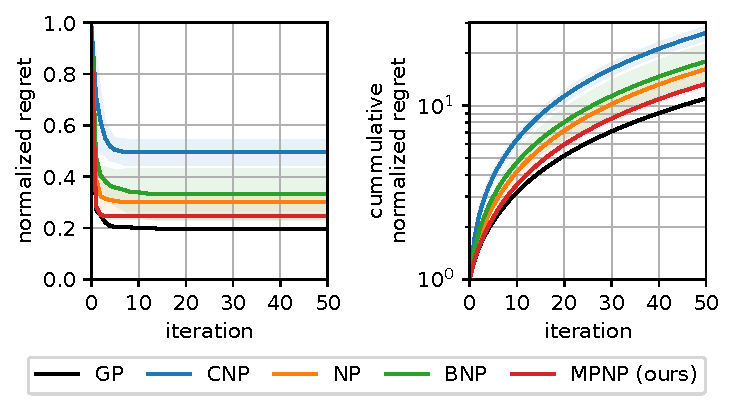
\includegraphics[width=0.49\linewidth]{figure/main_bo_gram_np}
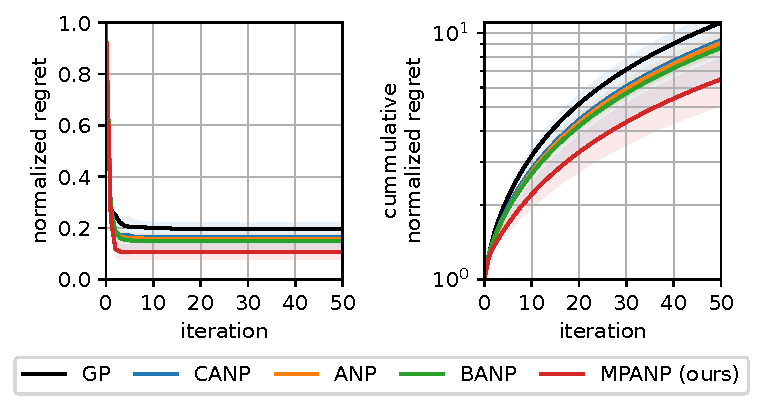
\includegraphics[width=0.49\linewidth]{figure/main_bo_gram_anp}
\caption{Results for Bayesian optimization on \citet{gramacy2012cases} function; we measured normalized simple regret and its cumulative value for a iteration. All models are pre-trained on 1D regression task generated with RBF kernel (cf.~\cref{main:sec:experiments:1dregression}) and evaluated on the benchmark function for Bayesian optimization.}
\label{figure/main_bo_gram}
\end{figure}


% \begin{figure}[t]
%     \centering
%     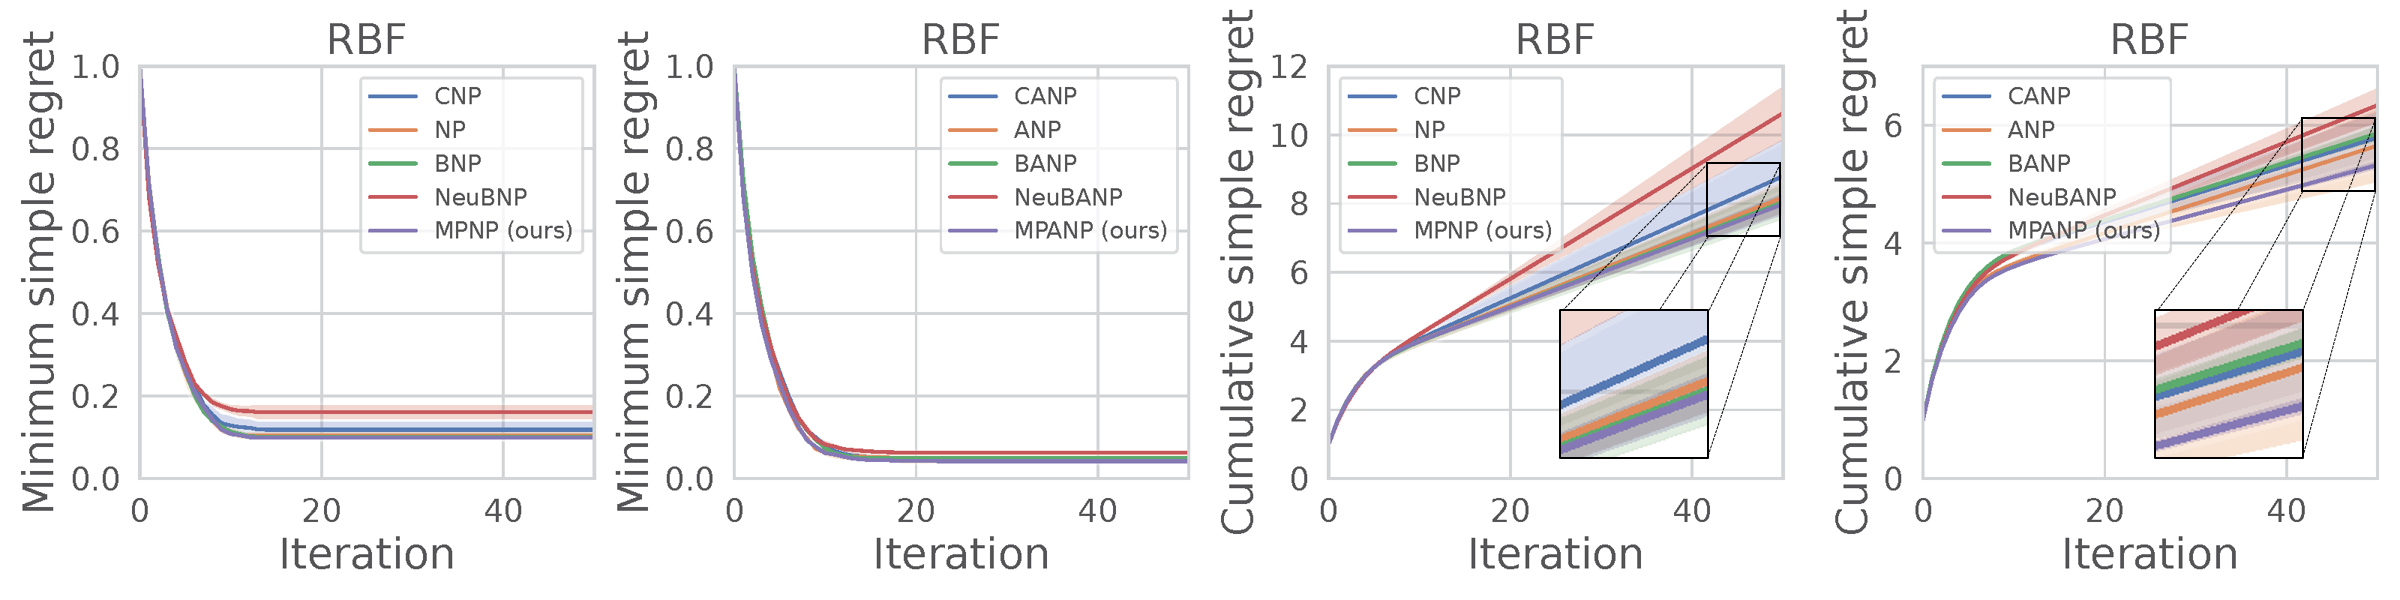
\includegraphics[width=0.95\textwidth]{figure/BO.png}
%     \caption{Results for Bayesian optimization with RBF kernel. Here we used 50 iterations for each model and report the means and standard deviations of minimum simple regret and cumulative simple regret for each iteration. The first and the second figure present the minimum simple regret for the models. The third and the forth figure present the cumulative simple regret for the models.}
%     \label{fig:figure_BO}
% \end{figure}
% We conducted Bayesian optimization~\citep{brochu2010tutorial} with tasks sampled from a \gls{gp} prior with RBF kernels. 
% We used pretrained models with RBF kernels in \cref{main:subsec:infinite_training} Infinite Training Dataset experiments.
% In Bayesian optimization, we use best simple regret, which measures the difference between current best value and the global optimum value, as a performance measurement.
% Following \citet{lee2020bootstrapping}, we evaluate the best simple regret and the cumulative best simple regret for 100 tasks.
% We used same fixed tasks and normalized initial minimum simple regret for the fare comparison among various models.
% In \cref{fig:figure_BO}, one can see that our model shows the best performance for both the best simple regret and especially on the cumulative best simple regret.

%%%%%%%%%%%%%%%%%%%%%%%%%%%%%%%%%%%%%%%%%%%%%%%%%%
\subsection{Predator-Prey Model}
\label{main:subsec:predator-prey}
Following~\citet{lee2020bootstrapping}, we conducted the predator-prey population regression experiments. We first trained the models using the simulation datasets which are generated from a Lotka-Volterra model~\citep{wilkinson2018stochastic} with the simulation settings followed by~\citet{lee2020bootstrapping}. Then tested on the generated simulation test dataset and real-world dataset which is called Hudson's Bay hare-lynx data. As mentioned in~\citet{lee2020bootstrapping}, the real-world dataset shows different tendency from generated simulation datasets, so we can treat this experiment as model-data mismatch experiments. In~\cref{table/main_lv}, we can see the \glspl{mpnp} outperform the other baselines for the test simulation datasets but underperforms in the real-world dataset compare to other baselines. This shows that model-data mismatch is an open problem for the \glspl{mpnp}.

\begin{table}[t]
\centering
\caption{Test results for predator-prey population regression tasks on Lotka-Volterra simulated data and real data. `Context' and `Target' respectively denote context and target log-likelihood values, and `Task' denotes the task log-likelihood. All values are averaged over four seeds.}
\label{table/main_lv}
\resizebox{0.8\linewidth}{!}{
\begin{tabular}{lrrrrrr}
\toprule
      & \multicolumn{3}{c}{Simulated data} & \multicolumn{3}{c}{Real data} \\
\cmidrule(lr){2-4}\cmidrule(lr){5-7}
Model & Context & Target & Task & Context & Target & Task \\
\midrule
CNP & 
 0.327$\spm{0.036}$ &  0.035$\spm{0.029}$ &  0.181$\spm{0.032}$ &
-2.686$\spm{0.024}$ & -3.201$\spm{0.042}$ & -3.000$\spm{0.034}$ \\
NP & 
 0.112$\spm{0.063}$ & -0.115$\spm{0.057}$ &  0.000$\spm{0.060}$ &
-2.770$\spm{0.028}$ & -3.144$\spm{0.031}$ & -2.993$\spm{0.029}$ \\
BNP & 
 0.550$\spm{0.057}$ &  0.274$\spm{0.042}$ &  0.417$\spm{0.050}$ &
\textBF{-2.614}$\spm{0.050}$ & \textBF{-3.052}$\spm{0.022}$ & \textBF{-2.868}$\spm{0.024}$ \\
\textBF{MPNP (ours)}  & 
 \textBF{0.626}$\spm{0.041}$ &  \textBF{0.375}$\spm{0.036}$ &  \textBF{0.500}$\spm{0.038}$ &
-2.621$\spm{0.072}$ & -3.092$\spm{0.054}$ & -2.918$\spm{0.061}$ \\
\midrule
CANP & 
 0.689$\spm{0.046}$ &  1.615$\spm{0.026}$ &  1.023$\spm{0.018}$ &
-4.743$\spm{1.119}$ & -6.413$\spm{0.339}$ & -5.801$\spm{0.733}$ \\
ANP & 
 2.607$\spm{0.015}$ &  1.830$\spm{0.020}$ &  2.234$\spm{0.018}$ &
 1.887$\spm{0.078}$ & -4.848$\spm{0.385}$ & -1.615$\spm{0.188}$ \\
BANP & 
 \textBF{2.654}$\spm{0.000}$ &  1.797$\spm{0.012}$ &  2.240$\spm{0.006}$ &
 \textBF{2.190}$\spm{0.062}$ & \textBF{-3.597}$\spm{0.279}$ & \textBF{-0.741}$\spm{0.160}$ \\
\textBF{MPANP (ours)} & 
 2.639$\spm{0.008}$ &  \textBF{1.835}$\spm{0.004}$ &  \textBF{2.254}$\spm{0.006}$ &
 1.995$\spm{0.145}$ & -5.073$\spm{0.680}$ & -1.690$\spm{0.401}$ \\
\bottomrule
\end{tabular}}
\end{table}


